\subsection{Space Decomposition}
\label{sec:spaceDec}

To perform a path planning and define a metric for deciding when a coverage is complete we have to sub-sample the space using a methodical approach. The most common approach is to apply a so called \emph{cellular decomposition} to the space. A mathematical definition of cellular decomposition is given in definition \ref{cellDec}.

\theoremstyle{definition}
\begin{definition}{\textbf{\textit{Cellular decomposition}}}\label{cellDec}
In geometric topology, a cellular decomposition $G$ of a manifold $M$ is a decomposition of $M$ as the disjoint union of cells (spaces homeomorphic to n-balls $B_n$).
\end{definition}

Practically a cellular decomposition is a data structure that encodes the topology of a given environment, using elementary non-overlapping regions of terrain of known geometry such that adjacent cells share a common boundary and that the union of all cells coincides with the environment. The main purpose of the decomposition is to derive an abstract description of the free space, i.e., the one in which the robot can move. Moving from cell to cell and covering the space in each cell for all of them will result in covering the entire region.
\clearpage
\noindent We can distinguish two types of cellular decomposition:
\begin{enumerate}
\item Exact cell decomposition (topology-dependent)
\item Approximate cell decomposition (topology-independent)
\end{enumerate}


In the exact cell decomposition the topology of the environment is accurately represented and to accomplish this all the cells does not have to be the same size, but they contain only free space. The method also requires a complete description of the objects and a complex cell construction.  In approximate cell decomposition, the entire region is divided into equal sized cells. Any cell with any part of an obstacle in it is marked as invalid workspace. The cells do not necessarily have to be marked as empty or full, but can be represented by a fraction of the portion occupied. The approximation can be improved by increasing the resolution but this of course will increase the memory requirements if the entire grid is stored in memory. After the cells are created an adjacency graph can be produced where each vertex represents a cell and the edges represents the adjacency relationship between the cells. Then this adjacency graph is used by the algorithms to perform the path planning in order to complete the coverage.

In \cite{846365} the authors present some new examples of exact cellular decompositions whose cells are defined by critical points of Morse functions. Cellular decompositions have been widely used for planning a path between two points in the free space, but the motivating task for the work presented in this paper is coverage. Since the Morse functions define cells with “simple” structure, a planner can then use a cellular decomposition to achieve coverage by employing simple control strategies to cover each of the individual cells in the decomposition. A simple
control strategy can be back-and-forth motions, resulting in a farming style pattern.

\begin{figure}[t] 
  \label{fig:cellDec_typess} 
  \begin{minipage}[b]{0.5\linewidth}
    \centering
    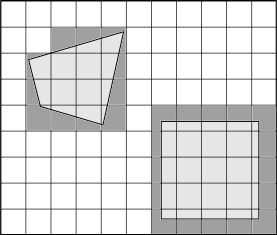
\includegraphics[width=0.7\textwidth]{approx_cell_decomp}
    \caption{Approx. cell decomposition}
    \label{fig:cellDec_pic1}
    \vspace{4ex}
  \end{minipage}
  \begin{minipage}[b]{0.5\linewidth}
    \centering
    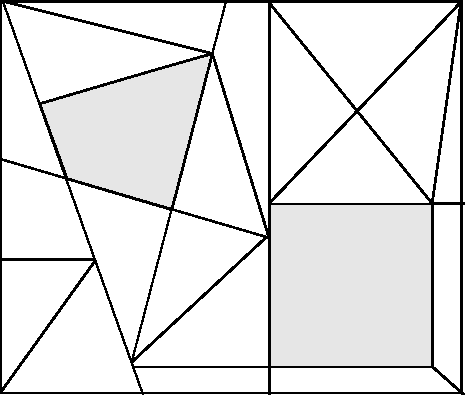
\includegraphics[width=0.7\textwidth]{exact_cell_decomp}
    \caption{Exact cell decomposition}
    \label{fig:cellDec_pic2}
    \vspace{4ex}%%
  \end{minipage}
  \begin{minipage}[b]{0.5\linewidth}
    \centering
    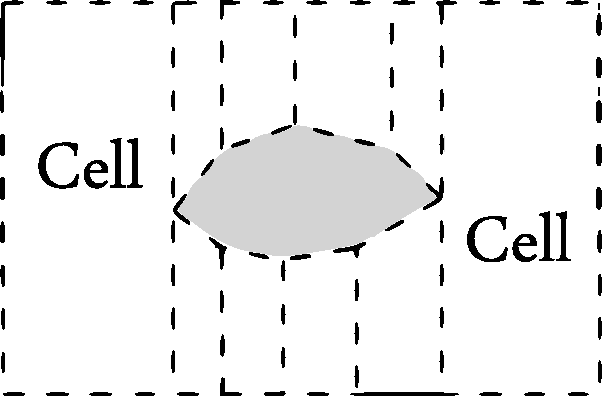
\includegraphics[width=0.7\textwidth]{trapezoidal_1}
    \caption{Trapezoidal decomposition} 
    \label{fig:cellDec_pic3}
    \vspace{4ex}
  \end{minipage}
  \begin{minipage}[b]{0.5\linewidth}
    \centering
    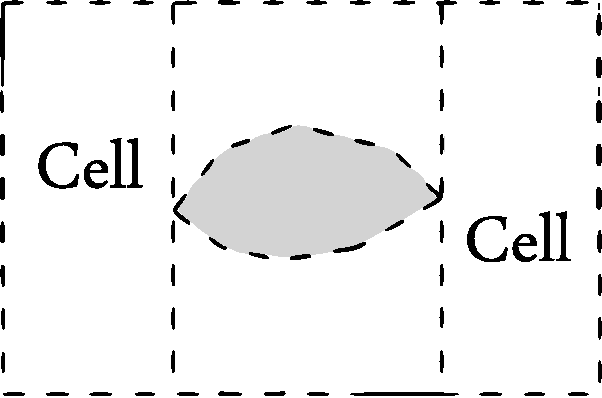
\includegraphics[width=0.7\textwidth]{boustrophedon_1}
    \caption{Boustrophedon decompostion}
    \label{fig:cellDec_pic4}
    \vspace{4ex}%% 
  \end{minipage} 
\end{figure}

In \cite{choset} the Boustrophedon Cellular Decomposition is introduced (figures \ref{fig:cellDec_pic3} and \ref{fig:cellDec_pic4}). Is an exact cellular decomposition approach, for the purposes of coverage. Essentially, the boustrophedon decomposition is a generalization of the trapezoidal decomposition that could allow for non-polygonal obstacles, but also has the side effect of having more “efficient” coverage paths than the trapezoidal decomposition. Cells are formed via a sequence of open and close operations which occur when the slice encounters an event, an instance in which a slice intersects a vertex of a polygon. There are three types of events: \emph{in}, \emph{out}, and \emph{middle}. Loosely speaking, at an \emph{in} event the current cell is closed (thereby completing its construction) and two new cells are opened (thereby initiating their construction). The boustrophedon cellular decomposition is an enhancement of the trapezoidal decomposition and is designed to minimize the number of excess lengthwise motions, as described in the previous paragraph. In essence, all cells between \emph{in} and \emph{out} events are merged into one cell. The advantage of having a fewer number of cells is that to complete the coverage the number of back-and-forth boustrophedon motions can be minimized. 

\begin{figure}[t] 
  \label{fig:grid_types} 
  \begin{minipage}[b]{0.5\linewidth}
    \centering
    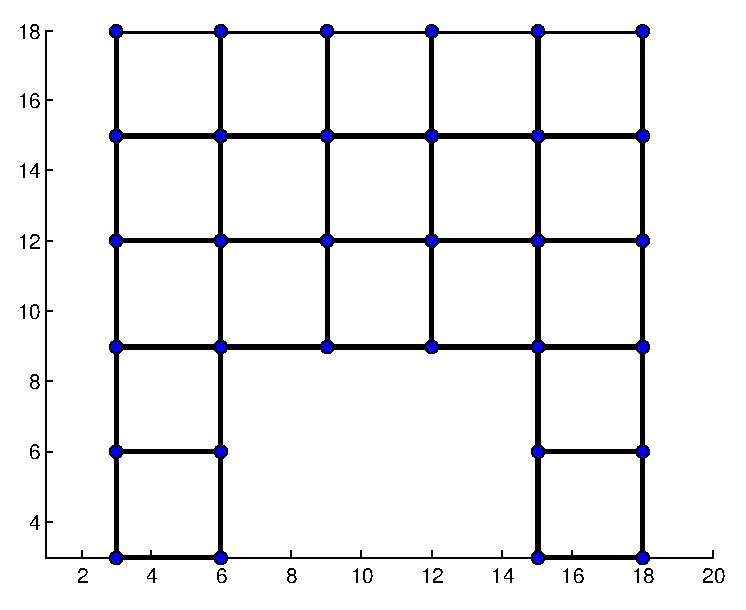
\includegraphics[width=0.7\textwidth]{6x6_Sparse1_1}
    \caption{Simple grid}
    \label{fig:grid1}
    \vspace{4ex}
  \end{minipage}
  \begin{minipage}[b]{0.5\linewidth}
    \centering
    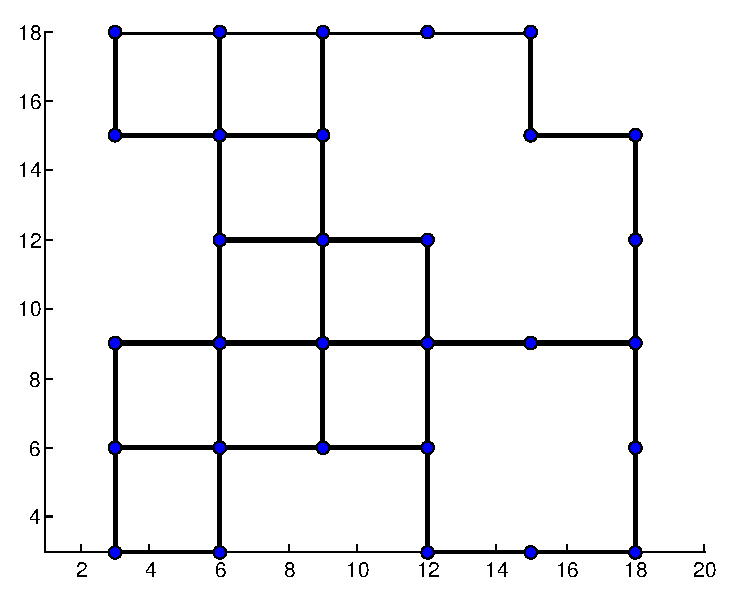
\includegraphics[width=0.7\textwidth]{6x6_Sparse2_1}
    \caption{Non-simple grid w/o l.c.n.}
    \label{fig:grid2}
    \vspace{4ex}%%
  \end{minipage}
\end{figure}

Regarding the approximate cell decomposition instead the logic is much simpler, since the only decision we have to make is how much we want the grid to be detailed. Then we mark as free only the cells that not contain any obstacle and all the rest as non-accessible space. In \cite{stanf:cellDec} a recursive strategy is presented where the cells are continuously subdivided until one of the following scenarios occurs: each cell lies either completely in free space or completely in the C-obstacle region, an arbitrary limit resolution is reached.
Once a cell fulfils one of these criteria, it stops decomposing. This method is also called a \emph{quadtree decomposition} because a cell is divided into four smaller cells of the same shape each time it gets decomposed.

Among the resulting grids we can distinguish between \mbox{\textit{simple grids}} (i.e., without internal holes) and \textit{non--simple grids} which do not possess \textit{local cut nodes} (i.e., nodes whose removal locally disconnects the graph induced by the grid). 


Both exact cell decomposition methods and approximate cell decomposition methods have advantages and disadvantages. The former are guaranteed to be complete, meaning that if a free path exists, exact cell decomposition will find it; however, the trade-off for this accuracy is a more difficult mathematical process. Approximate cell decomposition is less involved, but can yield similar, if not exactly the same, results as exact cell decomposition.

